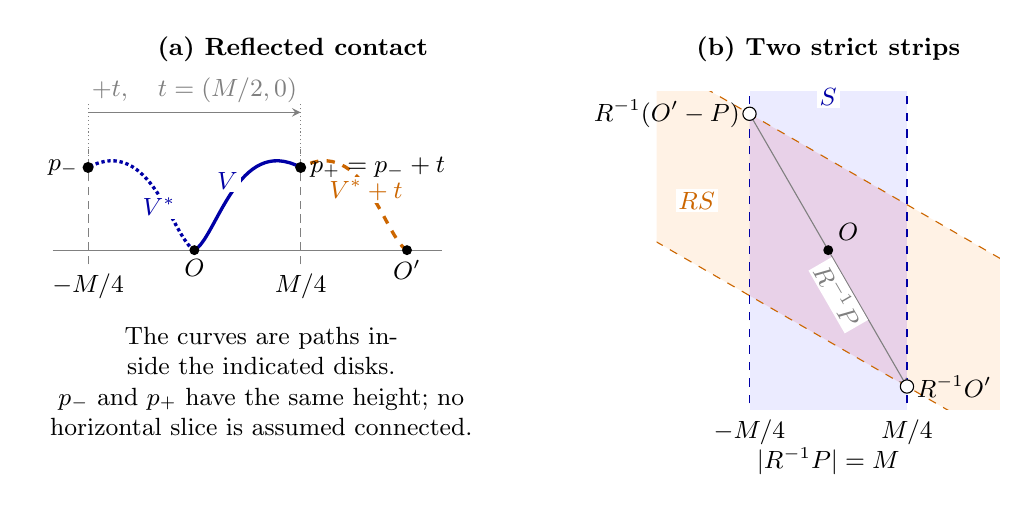
\begin{tikzpicture}[x=1cm,y=1cm,>=stealth,font=\small]
 \begin{scope}[shift={(2.4,0)}]
  \node[font=\small\bfseries] at (1.25,2.55) {(a) Reflected contact};
  \draw[gray] (-1.8,0)--(3.15,0);
  \draw[densely dashed,gray] (-1.35,-.18)--(-1.35,1.28);
  \draw[densely dashed,gray] (1.35,-.18)--(1.35,1.28);
  \draw[very thick,blue!65!black]
    (0,0) .. controls (.28,.15) and (.55,1.48) .. (1.35,1.05);
  \draw[very thick,blue!65!black,densely dotted]
    (0,0) .. controls (-.28,.15) and (-.55,1.48) .. (-1.35,1.05);
  \draw[very thick,orange!80!black,dashed]
    (2.7,0) .. controls (2.42,.15) and (2.15,1.48) .. (1.35,1.05);
  \draw[densely dotted,gray] (-1.35,1.05)--(-1.35,1.85);
  \draw[densely dotted,gray] (1.35,1.05)--(1.35,1.85);
  \draw[->,gray] (-1.35,1.75)--(1.35,1.75)
    node[midway,above] {$+t,\quad t=(M/2,0)$};
  \fill (0,0) circle (1.8pt) node[below] {$O$};
  \fill (2.7,0) circle (1.8pt) node[below] {$O'$};
  \fill (-1.35,1.05) circle (2pt)
    node[left] {$p_-$};
  \fill (1.35,1.05) circle (2pt)
    node[right] {$p_+=p_-+t$};
  \node[below] at (-1.35,-.18) {$-M/4$};
  \node[below] at (1.35,-.18) {$M/4$};
  \node[blue!65!black,fill=white,inner sep=1pt] at (.42,.88) {$V$};
  \node[blue!65!black,fill=white,inner sep=1pt] at (-.45,.55) {$V^*$};
  \node[orange!80!black,fill=white,inner sep=1pt] at (2.18,.76) {$V^*+t$};
  \node[anchor=north,align=center,text width=5.7cm] at (.85,-.85)
    {The curves are paths inside the indicated disks.\\
     \(p_-\) and \(p_+\) have the same height; no horizontal
     slice is assumed connected.};
 \end{scope}
 \begin{scope}[shift={(10.45,0)}]
  \node[font=\small\bfseries] at (0,2.55) {(b) Two strict strips};
  \begin{scope}
   \clip (-2.18,-2.02) rectangle (2.18,2.02);
   \fill[blue!8] (-1,-3) rectangle (1,3);
   \begin{scope}[rotate=60]
    \fill[orange!10] (-1,-3) rectangle (1,3);
   \end{scope}
   \fill[violet!18]
     (1,.57735)--(1,-1.73205)--(-1,-.57735)--(-1,1.73205)--cycle;
   \draw[blue!65!black,dashed] (-1,-3)--(-1,3);
   \draw[blue!65!black,dashed] (1,-3)--(1,3);
   \begin{scope}[rotate=60]
    \draw[orange!80!black,dashed] (-1,-3)--(-1,3);
    \draw[orange!80!black,dashed] (1,-3)--(1,3);
   \end{scope}
  \end{scope}
  \draw[->,gray] (-1,1.73205)--(1,-1.73205)
    node[pos=.64,sloped,below,fill=white,inner sep=1pt] {$R^{-1}P$};
  \fill (0,0) circle (1.8pt) node[above right] {$O$};
  \draw[fill=white] (-1,1.73205) circle (2.4pt)
    node[left] {$R^{-1}(O'-P)$};
  \draw[fill=white] (1,-1.73205) circle (2.4pt)
    node[right] {$R^{-1}O'$};
  \node[blue!65!black,fill=white,inner sep=1pt] at (0,1.95) {$S$};
  \node[orange!80!black,fill=white,inner sep=1pt] at (-1.67,.63) {$RS$};
  \node[below] at (-1,-2.03) {$-M/4$};
  \node[below] at (1,-2.03) {$M/4$};
  \node at (0,-2.68) {$|R^{-1}P|=M$};
 \end{scope}
\end{tikzpicture}
